\documentclass[a4paper]{article}

\usepackage[english]{babel}
\usepackage[utf8]{inputenc}
\usepackage[titletoc, toc]{appendix}
\usepackage{amsmath}
\usepackage{graphicx}
\usepackage{mdframed}
\usepackage{cancel}
\usepackage{caption}
\usepackage{lipsum}
\usepackage{listings}
\usepackage{float}
\usepackage{csvsimple}
\usepackage{array}
\usepackage[table]{xcolor}
\usepackage[colorinlistoftodos]{todonotes}

\definecolor{mGreen}{rgb}{0,0.6,0}
\definecolor{mGray}{rgb}{0.5,0.5,0.5}
\definecolor{mPurple}{rgb}{0.58,0,0.82}
\definecolor{backgroundColour}{rgb}{0.95,0.95,0.92}

\title{ACM40640 High Performance Comp \\ Assignment 1}

\author{Ian Towey \\ \\ 04128591}

\date{\today}

\lstdefinestyle{custom_py_style}{
  belowcaptionskip=1\baselineskip,
  breaklines=true,
  frame=L,
  xleftmargin=\parindent,
  language=Python,
  showstringspaces=false,
  basicstyle=\footnotesize\ttfamily,
  keywordstyle=\bfseries\color{green!40!black},
  commentstyle=\itshape\color{purple!40!black},
  identifierstyle=\color{blue},
  stringstyle=\color{orange}
}

\lstdefinestyle{CStyle}{
    backgroundcolor=\color{backgroundColour},   
    commentstyle=\color{mGreen},
    keywordstyle=\color{magenta},
    numberstyle=\tiny\color{mGray},
    stringstyle=\color{mPurple},
    basicstyle=\footnotesize,
    breakatwhitespace=false,         
    breaklines=true,                 
    captionpos=t,                    
    keepspaces=true,                 
    numbers=left,                    
    numbersep=5pt,                  
    showspaces=false,                
    showstringspaces=false,
    showtabs=false,                  
    tabsize=2,
    language=C
}


% Number the subsubsections and include them in the TOC
\setcounter{secnumdepth}{3}
\setcounter{tocdepth}{3}
\setcounter{section}{-1}

\begin{filecontents*}{a500.csv}
name,givenname,matriculation,gender,grade
500,1,0.136818,1,1
500,5,0.032769,0.239507959479016,4.17522658610272
500,10,0.03897,0.284830943296935,3.5108545034642
500,15,0.061737,0.451234486690348,2.21614266971184
500,20,0.109617,0.801188440117528,1.24814581679849
500,25,0.094764,0.692628162961014,1.44377611751298
500,30,0.085122,0.622154979607946,1.60731655741172
500,35,0.074294,0.543013346197138,1.841575362748
500,40,0.061368,0.448537473139499,2.22946812671099
\end{filecontents*}

\begin{filecontents*}{a1000.csv}
name,givenname,matriculation,gender,grade
1000,1,8.32384,1,1
1000,5,1.789278,0.214958240427495,4.6520663641983
1000,10,0.98218,0.1179960210672,8.47486204158097
1000,15,0.670694,0.0805750711210211,12.4107864391213
1000,20,0.627197,0.0753494781254805,13.2714920511418
1000,25,0.687821,0.0826326551207135,12.1017532177703
1000,30,0.638659,0.0767264868137783,13.0333088549602
1000,35,0.546503,0.0656551543518376,15.2310966270999
1000,40,0.499063,0.0599558617176688,16.6789363266762
\end{filecontents*}

\begin{filecontents*}{a2000.csv}
name,givenname,matriculation,gender,grade
2000,1,81.919144,1,1
2000,5,17.612401,0.214997375949143,4.65121955831008
2000,10,9.42893,0.1151004458738,8.68806365091267
2000,15,6.309168,0.0770170157051446,12.9841437095985
2000,20,4.834022,0.0590096742221818,16.9463738476987
2000,25,5.673005,0.0692512729381059,14.4401677770423
2000,30,4.915481,0.0600040571713005,16.6655397508403
2000,35,4.304687,0.0525479978159928,19.0302207802797
2000,40,4.444649,0.0542565361766964,18.4309591151067
\end{filecontents*}

\begin{filecontents*}{a3000.csv}
name,givenname,matriculation,gender,grade
3000,1,379.905421,1,1
3000,5,72.595633,0.191088699942505,5.23317182178162
3000,10,38.912887,0.102427827688197,9.76297186584999
3000,15,26.133908,0.0687905635334433,14.5368775691718
3000,20,19.820675,0.0521726564149239,19.1671283142476
3000,25,21.94133,0.057754716798316,17.3146031256993
3000,30,19.670081,0.0517762577544267,19.3138717120687
3000,35,17.172593,0.0452022847023286,22.1227755761754
3000,40,17.271112,0.0454616097726071,21.9965814013597
\end{filecontents*}

\begin{filecontents*}{a4000.csv}
name,givenname,matriculation,gender,grade
4000,1,732.608332,1,1
4000,5,183.152083,0.25,4
4000,10,102.377162,0.139743376546801,7.15597422010976
4000,15,67.713204,0.0924275646922345,10.8192832228113
4000,20,51.827723,0.0707441080536332,14.1354527961801
4000,25,55.588827,0.0758779617592446,13.1790572231359
4000,30,50.389406,0.0687808257141143,14.5389356643736
4000,35,43.283283,0.0590810684364425,16.9258956627666
4000,40,42.753439,0.0583578388786329,17.1356585373167
\end{filecontents*}

\begin{filecontents*}{a5000.csv}
name,givenname,matriculation,gender,grade
5000,1,1548.988168,1,1
5000,5,387.247042,0.25,4
5000,10,209.308222,0.135125771987175,7.40051276151015
5000,15,141.228929,0.0911749566056078,10.9679240575421
5000,20,107.211277,0.0692137481840339,14.4479966225941
5000,25,111.409326,0.0719239360903885,13.9035772283552
5000,30,105.991707,0.0684264148620663,14.6142392819468
5000,35,97.041795,0.0626485062989842,15.9620725070059
5000,40,93.206691,0.0601726294141712,16.618851623002
\end{filecontents*}


\newenvironment{aside}
  {\begin{mdframed}[style=0,%
      leftline=false,rightline=false,leftmargin=2em,rightmargin=2em,%
          innerleftmargin=0pt,innerrightmargin=0pt,linewidth=0.5pt,%
      skipabove=7pt,skipbelow=7pt]\footnotesize}
  {\end{mdframed}}

\begin{document}

  \maketitle

  \begin{abstract}
    OpenMP code analysis
  \end{abstract}

\tableofcontents

\newpage
\section{Matrix-Matrix Multiplication}

This section analyses matrix mutliplcation performance using OpenMP on the fionn HPC at ICHEC. 

The OpenMP pragma to parallelise this program is
\lstinputlisting[language=Python,style=CStyle, firstline=59, lastline=67]{/home/ian/Desktop/ACM40640-High-Performance-Comp/Assignment1/fionn/code/q1/main.c}

After logging onto To initialise environment run

\begin{verbatim}
 $ cd /ichec/home/users/ph5xx10/PH504/assignment1/code/q1
 $ . setenv
 $ qsub -I -l walltime=00:20:00 -l nodes=3:ppn=24 -N mma -j oe -r n -A ph5xx
\end{verbatim}

Script compile\_run.sh takes two parameters in the following order

\begin{itemize}
 \item Matrix Dimension (integer)
 \item Number of runs (integer) - this is used to run the matrix multiplcation operation N times and then average run time is reported (total\_time\_for\_N\_runs/ N)
\end{itemize}

The script compiles the program main.c and runs the matrix multiplcation program for 1, 5, 10, 15, 20, 25, 30, 35, 40 threads, Below is a sample run and output from local laptop with 8 cores

\begin{verbatim}
 $ sh compile_run.sh 500 1
******************************************************************
*thread count, Matrix Dimension, Number of runs, Avg run time
******************************************************************
1,500,1,0.158027
******************************************************************
******************************************************************
*thread count, Matrix Dimension, Number of runs, Avg run time
******************************************************************
5,500,1,0.046936
******************************************************************
******************************************************************
*thread count, Matrix Dimension, Number of runs, Avg run time
******************************************************************
10,500,1,0.043478
******************************************************************
******************************************************************
*thread count, Matrix Dimension, Number of runs, Avg run time
******************************************************************
15,500,1,0.042990
******************************************************************
******************************************************************
*thread count, Matrix Dimension, Number of runs, Avg run time
******************************************************************
20,500,1,0.049902
******************************************************************
******************************************************************
*thread count, Matrix Dimension, Number of runs, Avg run time
******************************************************************
25,500,1,0.042828
******************************************************************
******************************************************************
*thread count, Matrix Dimension, Number of runs, Avg run time
******************************************************************
30,500,1,0.044276
******************************************************************
******************************************************************
*thread count, Matrix Dimension, Number of runs, Avg run time
******************************************************************
35,500,1,0.043903
******************************************************************
******************************************************************
*thread count, Matrix Dimension, Number of runs, Avg run time
******************************************************************
40,500,1,0.042143
******************************************************************

\end{verbatim}

Executing the script on fionn for various dim sizes
\begin{verbatim}
$ qsub -I -l walltime=00:20:00 -l nodes=3:ppn=24 -N mma -j oe -r n -A ph5xx
$ sh compile_run.sh 500 1
\end{verbatim}

\noindent\begin{tabular}{|c|c|c|}
\hline
\rowcolor{lightgray}\multicolumn{3}{ |c| }{\bfseries Matrix Dim : 500} \\
\hline
\bfseries No. Threads & \bfseries Time Taken (s) & \bfseries Relative speedup% specify table head
\csvreader[head to column names]{a500.csv}{}% use head of csv as column names
{\\\hline\givenname & \matriculation & \grade}% specify your coloumns here
\\\hline
\end{tabular}

\begin{verbatim}
$ qsub -I -l walltime=00:20:00 -l nodes=3:ppn=24 -N mma -j oe -r n -A ph5xx
$ sh compile_run.sh 1000 1
\end{verbatim}

\noindent\begin{tabular}{|c|c|c|}
\hline
\rowcolor{lightgray}\multicolumn{3}{ |c| }{\bfseries Matrix Dim : 1000} \\
\hline
\bfseries No. Threads & \bfseries Time Taken (s) & \bfseries Relative speedup% specify table head
\csvreader[head to column names]{a1000.csv}{}% use head of csv as column names
{\\\hline\givenname & \matriculation & \grade}% specify your coloumns here
\\\hline
\end{tabular}

\begin{verbatim}
$ qsub -I -l walltime=00:20:00 -l nodes=3:ppn=24 -N mma -j oe -r n -A ph5xx
$ sh compile_run.sh 2000 1
\end{verbatim}
\noindent\begin{tabular}{|c|c|c|}
\hline
\rowcolor{lightgray}\multicolumn{3}{ |c| }{\bfseries Matrix Dim : 2000} \\
\hline
\bfseries No. Threads & \bfseries Time Taken (s) & \bfseries Relative speedup% specify table head
\csvreader[head to column names]{a2000.csv}{}% use head of csv as column names
{\\\hline\givenname & \matriculation & \grade}% specify your coloumns here
\\\hline
\end{tabular}

\begin{verbatim}
$ qsub -I -l walltime=00:20:00 -l nodes=3:ppn=24 -N mma -j oe -r n -A ph5xx
$ sh compile_run.sh 3000 1
\end{verbatim}
\noindent\begin{tabular}{|c|c|c|}
\hline
\rowcolor{lightgray}\multicolumn{3}{ |c| }{\bfseries Matrix Dim : 3000} \\
\hline
\bfseries No. Threads & \bfseries Time Taken (s) & \bfseries Relative speedup% specify table head
\csvreader[head to column names]{a3000.csv}{}% use head of csv as column names
{\\\hline\givenname & \matriculation & \grade}% specify your coloumns here
\\\hline
\end{tabular}

\begin{verbatim}
$ qsub -I -l walltime=00:20:00 -l nodes=3:ppn=24 -N mma -j oe -r n -A ph5xx
$ sh compile_run.sh 4000 1
\end{verbatim}

\noindent\begin{tabular}{|c|c|c|}%
\hline
\rowcolor{lightgray}\multicolumn{3}{ |c| }{\bfseries Matrix Dim : 4000} \\
\hline
\bfseries No. Threads & \bfseries Time Taken (s) & \bfseries Relative speedup% specify table head
\csvreader[head to column names]{a4000.csv}{}% use head of csv as column names
{\\\hline\givenname & \matriculation & \grade}% specify your coloumns here
\\\hline
\end{tabular}

\begin{verbatim}
$ qsub -I -l walltime=00:20:00 -l nodes=3:ppn=24 -N mma -j oe -r n -A ph5xx
$ sh compile_run.sh 5000 1
\end{verbatim}

\noindent\begin{tabular}{|c|c|c|}%
\hline
\rowcolor{lightgray}\multicolumn{3}{ |c| }{\bfseries Matrix Dim : 5000} \\
\hline
\bfseries No. Threads & \bfseries Time Taken (s) & \bfseries Relative speedup% specify table head
\csvreader[head to column names]{a5000.csv}{}% use head of csv as column names
{\\\hline\givenname & \matriculation & \grade}% specify your coloumns here
\\\hline
\end{tabular}

\vspace{5mm}

Below chart shows almost linear speed up of the matrix maltuiplication using OpenMP pragmas up to about 20 threads, then the benefit of mutlithread processing 
deminishes significately

\begin{figure}[H]
\centering
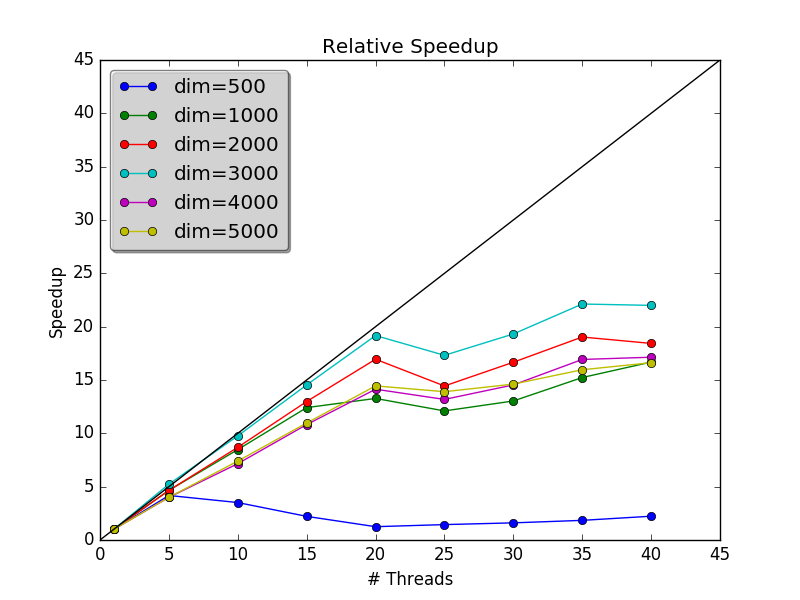
\includegraphics[width=1\textwidth]{/home/ian/Desktop/ACM40640-High-Performance-Comp/Assignment1/Relative_Speedup.png}
\caption{\label{fig:data}Relative Speed}
\end{figure}


\newpage
\section{Area under a curve}

Calculating Area under a curve using the trapezoid rules and OpenMP

\begin{verbatim}
 $ cd /ichec/home/users/ph5xx10/PH504/assignment1/code/q2
 $ . setenv
 $ qsub -I -l walltime=00:20:00 -l nodes=3:ppn=24 -N mma -j oe -r n -A ph5xx
\end{verbatim}

Example output of running 
\begin{verbatim}
 $ sh compile_run.sh 
***********************************************************
*Threads count ,Runs, Avg_loop_time/Runs, Computed area
***********************************************************
1, 1, 2.39603304862976074219, 6.41113026187355483643
***********************************************************
***********************************************************
*Threads count ,Runs, Avg_loop_time/Runs, Computed area
***********************************************************
2, 1, 1.21004486083984375000, 6.41113026188736423450
***********************************************************
***********************************************************
*Threads count ,Runs, Avg_loop_time/Runs, Computed area
***********************************************************
4, 1, 0.62412595748901367188, 6.41113026188496260005
***********************************************************
\end{verbatim}


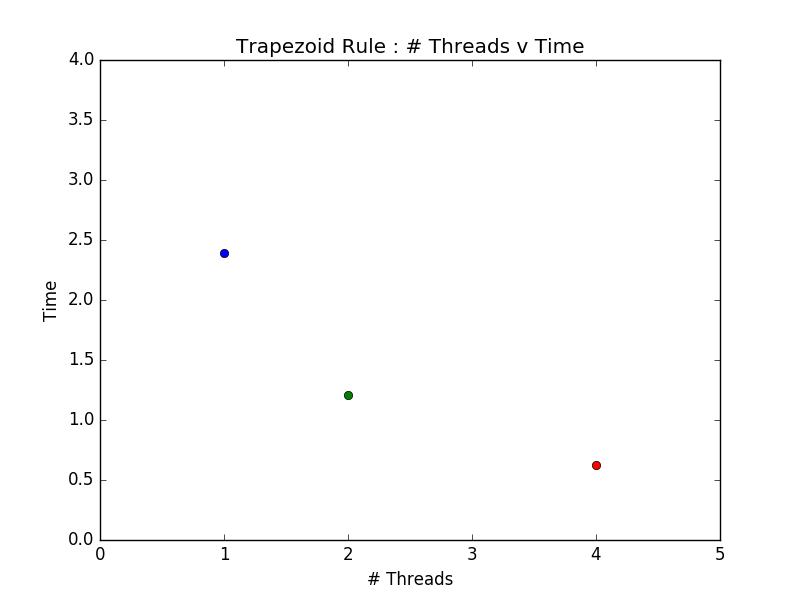
\includegraphics[width=1\textwidth]{/home/ian/Desktop/ACM40640-High-Performance-Comp/Assignment1/code/q2/Speedup.png}

\newpage
\section{Computing $\pi$ using Monte Carlo methods}

1. A Crtical section is identified to limit the impact of the threads on shared variable
 \lstinputlisting[language=Python,style=CStyle, firstline=19, lastline=36]{/home/ian/Desktop/ph504_ass1_q3/main.c}


2. The function ran3 is the thread safe implementation of ran2, it takes a seed as parameter , but returns a struct of the mutated seed and random value.

 \lstinputlisting[language=Python,style=CStyle, firstline=40, lastline=65]{/home/ian/Desktop/ph504_ass1_q3/main.c}

3. 

4.



\end{document}
